% -*- coding: UTF-8 -*-
% vim: autoindent expandtab tabstop=4 sw=4 sts=4 filetype=tex
% vim: spelllang=de spell
% chktex-file 27 - disable warning about missing include files

\section{Domänenmodell}
\label{sec:domain-model}

Der wesentliche Schritt der objektorientierten Analyse ist die Zerlegung einer
Domäne in essentielle Konzepte oder Objekte~\cite{larman_applying_2004}.

In UML wird ein Domänenmodell typischerweise als eine Menge von
Klassendiagrammen ohne Operationen dargestellt. Es liefert eine konzeptuelle
Perspektive und kann folgende Elemente beinhalten~\cite{larman_applying_2004}:
\begin{itemize}
    \item{Objekte der Domäne oder konzeptuelle Klassen}
    \item{Relationen zwischen konzeptuellen Klassen}
    \item{Attribute der konzeptuellen Klassen}
\end{itemize}

Da angedacht ist, dass die Applikation aus zwei Applikationen, dem
\textit{Player} sowie dem \textit{Editor}, besteht, wird für jede
Applikation ein Domänenmodell erstellt.

\subsection{Player}
\label{subsec:domain-model:player}

\begin{figure}[H]
    \centering
    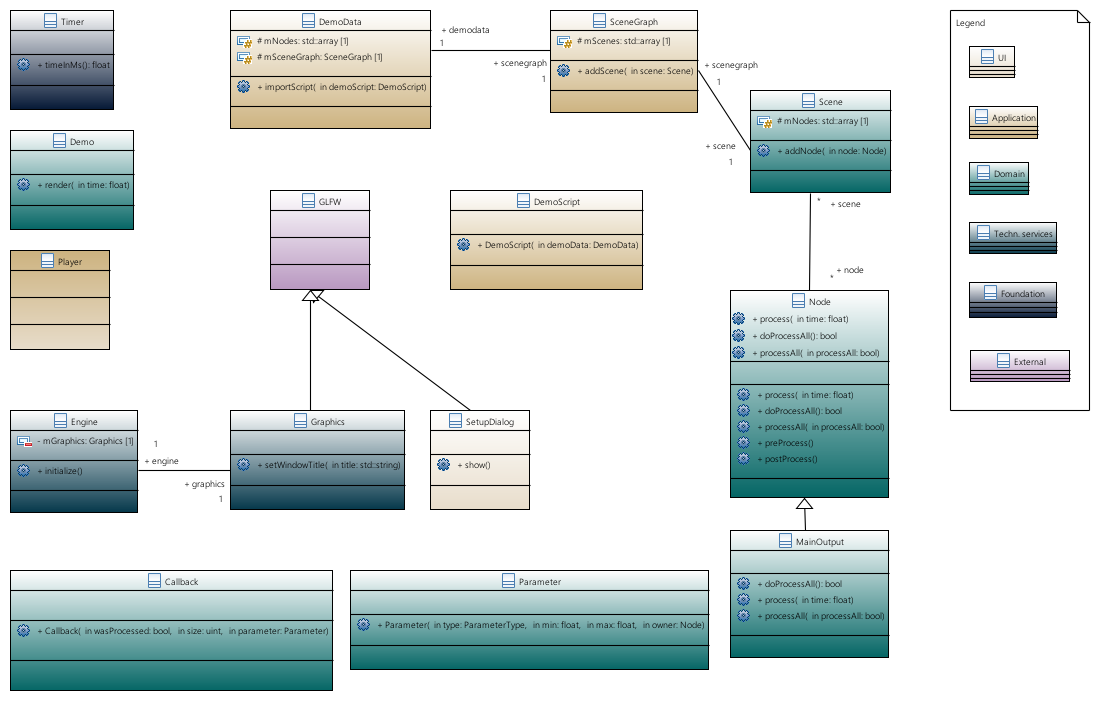
\includegraphics{img/player_class_diagram.pdf}
    \caption{Domänenmodell der
        Player-Applikation\protect\footnotemark}\label{fig:domain-model:player}
\end{figure}
\footnotetext{Eigene Darstellung mittels Papyrus.}

\todo[inline]{Describe player domain model.}

\subsection{Editor}
\label{subsec:domain-model:editor}

\begin{figure}[H]
    \centering
    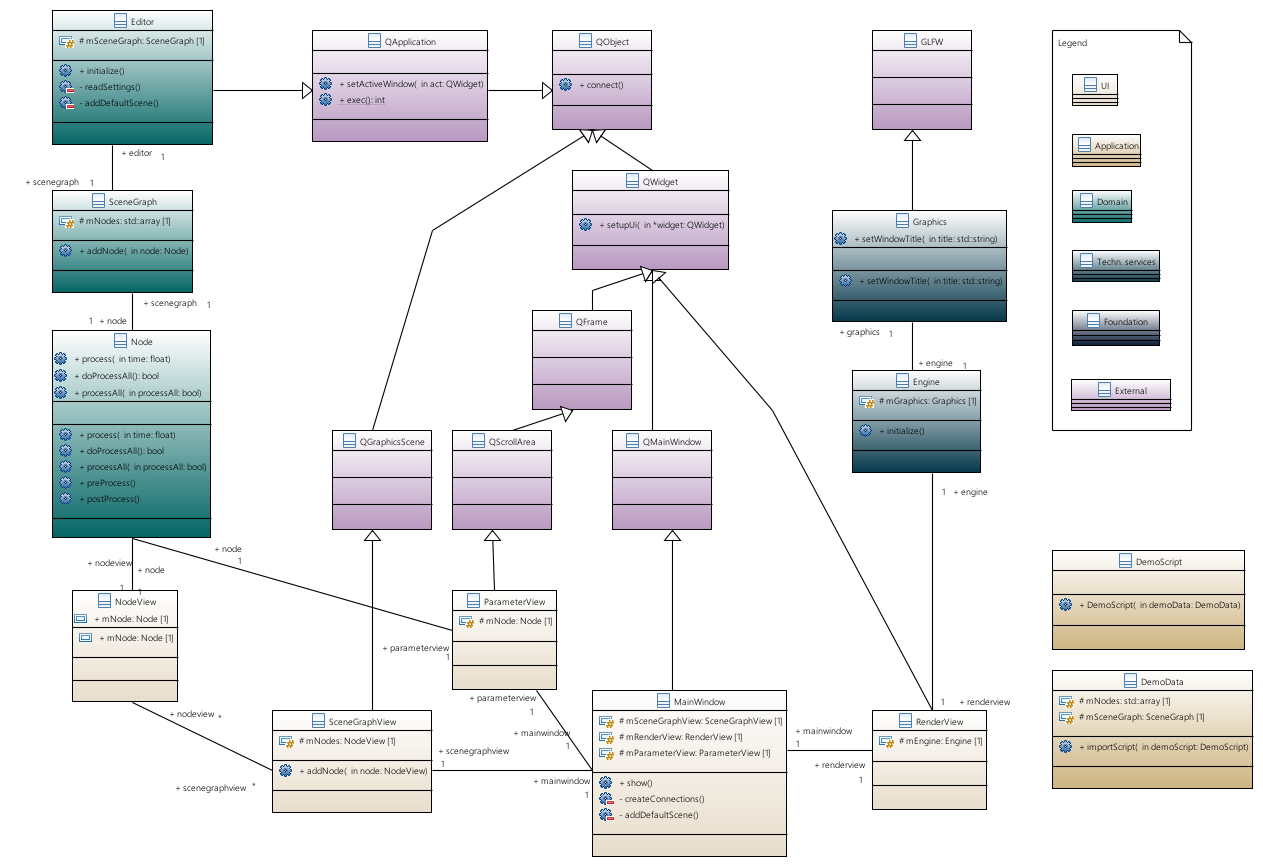
\includegraphics[angle=90,width=0.7\textwidth]{img/editor_class_diagram.pdf}
    \caption{Domänenmodell der
        Editor-Applikation\protect\footnotemark}\label{fig:domain-model:editor}
\end{figure}
\footnotetext{Eigene Darstellung mittels Papyrus.}

\todo[inline]{Describe editor domain model.}
